\documentclass[koma,a4paper]{article}
\usepackage[T1]{fontenc}
\usepackage{fixltx2e}
\usepackage{graphicx}
\usepackage{float}
\usepackage{amsmath}
\usepackage{amssymb}
\usepackage[hidelinks]{hyperref}
\usepackage{amsthm}
\usepackage{tikz}
\usepackage{todonotes}
\usepackage{booktabs}
\usepackage{subcaption}
\usepackage{color}
\usepackage{lmodern}
\usepackage{mathtools}
\usetikzlibrary{trees}
\usepackage[utf8]{inputenc}
\DeclarePairedDelimiter{\ceil}{\lceil}{\rceil}

\newcommand*\circled[1]{\tikz[baseline=(char.base)]{\node[shape=circle,draw,inner sep=2pt] (char) {#1};}} % circles around numbers

\title{AALG Self Study 6}
\author{Andreas Petersen\\
Mads E. Kalør\\
Søren B. Ranneries\\
Room 1.1.34}
\begin{document}
\maketitle

\pagebreak

\section{Exercise 1}
We can parallelize the two inner loops because they depend only on $k-1$. The outer loop must be executed in order, otherwise it will not work.
\begin{align*}
  &\text{Floyd-Warshall}(W)\\
  &~~~~n \leftarrow W.\text{rows}\\
  &~~~~D^{(0)} \leftarrow W\\
  &~~~~\text{for } k \leftarrow 1 \text{ to } n\\
  &~~~~~~~~D^{(k)} \leftarrow \text{new Matrix(}(d_{ij}^{(k)})\\
  &~~~~~~~~\text{parallel for } i \leftarrow 1 \text{ to } n\\
  &~~~~~~~~~~~~\text{parallel for } j \leftarrow 1 \text{ to } n\\
  &~~~~~~~~~~~~~~~~d_{ij}^{(k)} \leftarrow \text{min}(d_{ij}^{(k-1)}, d_{ik}^{(k-1)}, d_{kj}^{(k-1)})\\
  &~~~~\text{return } D^{(n)}\\
\end{align*}
Work: $\Theta(n^3)$. Span: $\Theta(n \lg^2 n)$. Parallelism: $\Theta(\frac{n^2}{\lg^2 n})$.

\section{Exercise 2}
\begin{align*}
  &\text{Parallel-Partitioning}(A[1..n])\\
  &~~~~x \leftarrow A[n] \\
  &~~~~L \leftarrow \text{new Array}[1..n]\\
  &~~~~S \leftarrow \text{new Array}[1..n]\\
  &~~~~\text{parallel for } i \leftarrow 1 \text{ to } n\\
  &~~~~~~~~\text{if } A[i] \leq x \text{ then}\\
  &~~~~~~~~~~~~S[i] \leftarrow A[i]\\
  &~~~~~~~~\text{else then}\\
  &~~~~~~~~~~~~L[i] \leftarrow A[i]\\
  &~~~~L' \leftarrow \text{Compact(L, 1, n)}\\
  &~~~~S' \leftarrow \text{Compact(S, 1, n)}\\
  &~~~~\text{parallel for } i \leftarrow 1 \text{ to } S'.\text{size}\\
  &~~~~~~~~A[i] \leftarrow S'[i]\\
  &~~~~\text{parallel for } i \leftarrow S'.\text{size}+1 \text{ to } n\\
  &~~~~~~~~A[i] \leftarrow L'[i]\\
  &~~~~\text{return } A\\
\end{align*}
Work: $3\Theta(n)+2\Theta(n \lg n) = \Theta(n \lg n)$. Span: $3\Theta(\lg n)+2\Theta(\lg^2 n)=\Theta(\lg^2 n)$. Parallelism: $\Theta(\frac{n}{\lg n})$.

\section{Exercise 3}
\subsection{A}
This is a maximal matching which is not a maximum matching (the dashed edges are in the set of edges):\\
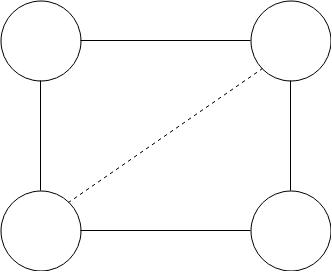
\includegraphics[width=0.4\textwidth]{graph1}\\
This is a maximum matching:\\
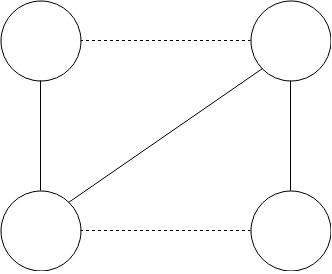
\includegraphics[width=0.4\textwidth]{graph2}\\
\subsection{B}
\begin{align*}
  &\text{Greedy-Maximal-Matching}(V,E)\\
  &~~~~E' \leftarrow \emptyset\\
  &~~~~\text{foreach } (u,v) \in E\\
  &~~~~\text{if u.marked} = \text{false and v.marked} = \text{false then}\\
  &~~~~~~~~E' \leftarrow E' \cup \{(u,v)\}\\
  &~~~~~~~~u.\text{marked} \leftarrow true\\
  &~~~~~~~~v.\text{marked} \leftarrow true\\
  &~~~~\text{return } E'\\
\end{align*}
\subsection{C}
From the definition of a matching follows that no edges in the maximum matching share endpoints. To cover all edges in the maximum matching with a vertex cover at least one of the endpoints of each edge needs to be in the vertex cover. Therefore the lower bound on the size of any vertex cover for a graph is the size of the maximum matching for that graph.
\subsection{D}
There are no edges left in the resulting subgraph.
\subsection{E}
$T$ is a vertex cover containing $2|M|$ vertices.
\subsection{F}
$$|M| \leq c(H^*) \leq c(H) \leq 2|M|$$
So because the solution is between $|M|$ and $2|M|$, it is a 2-approximation algorithm.
\end{document}
